
\begin{exercise}
Find the horizontal and vertical intercepts or state that they don't exist for each function given below.


\begin{parts}

\item $y=3x-1.5$

\item $f(x)=1-x^2$

\item $g(t)=5.4-0.2t$

\item $y=2x^3+16$

\item $h(m)=2\sqrt{m}-3$

\item $ y=\dfrac{1}{x}$

\item $\displaystyle y=\frac{1}{x-1}$

\end{parts}

\end{exercise}


\begin{solution}
    \begin{parts}
        \item {\bf horizontal intercept:} 0.5; {\bf vertical intercept:} $-1.5$
        \item {\bf horizontal intercepts:} $-1$, 1; {\bf vertical intercept:} 1
        \item {\bf horizontal intercept:} 27; {\bf vertical intercept:} 5.4
        \item {\bf horizontal intercept:} $-2$; {\bf vertical intercept:} 16
        \item {\bf horizontal intercept:} 9/4; {\bf vertical intercept:} $-3$
        \item {\bf horizontal intercepts:} none; {\bf vertical intercept:} none
        \item {\bf horizontal intercept:} none; {\bf vertical intercept:} $-1$
    \end{parts}
\end{solution}






\begin{exercise}
Identify the horizontal and vertical intercepts for each function given numerically below.


\begin{parts}
\item \begin{tabular}{|c|c|c|c|c|c|c|}
\hline $x$ &$-2$ & $-1$ & 0 & 1 & 2 & 3
\\\hline $y$ & 3 & 0  & 2 & 2.5  & 0 & 4 
\\\hline
\end{tabular}

\vspace{5pt}

\item \begin{tabular}{|c|c|c|c|c|c|c|}
\hline $t$ &0 & 2 & 4 & 6 & 8 & 10
\\\hline $f(t)$ & 5 & 6  & 8 & 4  & 8 & 4 
\\\hline
\end{tabular}

\vspace{5pt}

\item\begin{tabular}{|c|c|c|c|c|c|c|}
\hline $x$ &3 & 4 & 5 & 6 & 7 & 8
\\\hline $g(x)$ & $-5$ & $-4$  & $-5$ & $-2$  & $-2$ & 0 
\\\hline
\end{tabular}

\end{parts}
\end{exercise}



\begin{solution}
    \begin{parts}
        \item {\bf horizontal intercepts:} $-1$, 2; {\bf vertical intercept:} 2
        \item {\bf horizontal intercepts:} none; {\bf vertical intercept:} 5
        \item {\bf horizontal intercept:} 8; {\bf vertical intercept:} none
    \end{parts}
\end{solution}





\begin{exercise}
Estimate the horizontal and vertical intercepts for each function given graphically below.


\begin{parts}

\item 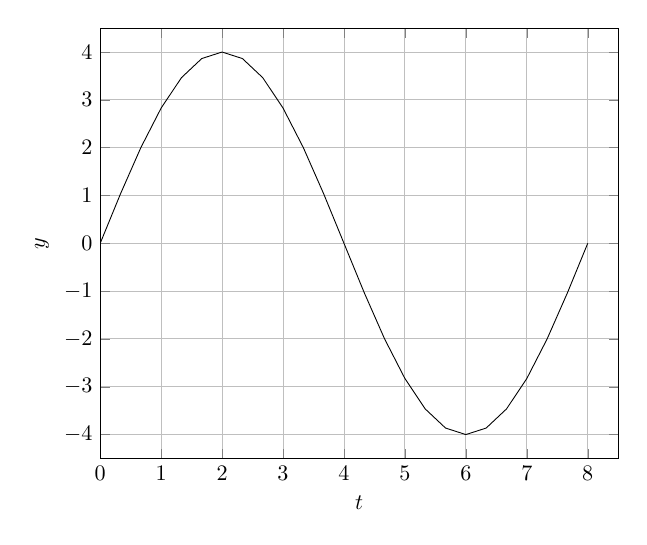
\begin{tikzpicture}[scale=0.8]
\begin{axis}[grid=both,
xmin=0,xmax=8.5,
ymin=-4.5,ymax=4.5,
xtick={0,1,...,8},
ytick={-4,...,4},
minor tick={},
xlabel=\(t\), ylabel=\(y\),
x post scale = 1.2,
y post scale = 1.2
]
\addplot[domain=0:8] {4*sin(2*pi/8*deg(x))};
\end{axis}
\end{tikzpicture}





\item 

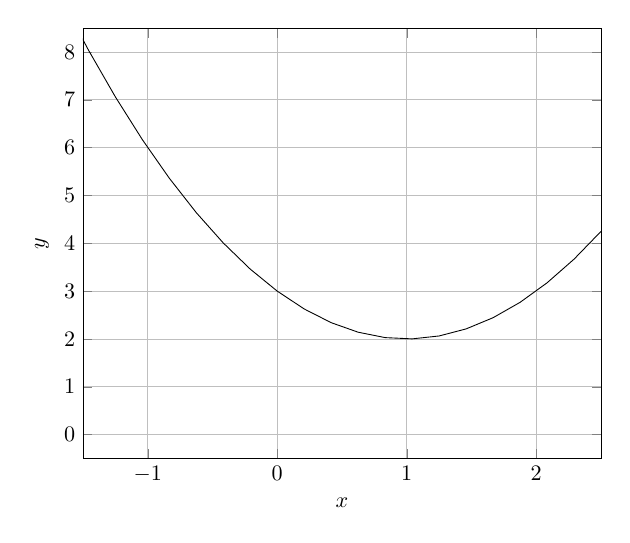
\begin{tikzpicture}[scale=0.8]
\begin{axis}[grid=both,
xmin=-1.5,xmax=2.5,
ymin=-0.5,ymax=8.5,
xtick={-2,-1,...,3},
ytick={-8,...,8},
minor tick={},
xlabel=\(x\), ylabel=\(y\),
x post scale = 1.2,
y post scale = 1.2
]
\addplot[domain=-2.5:2.5] {(x-1)^2+2};
\end{axis}
\end{tikzpicture}
\end{parts}

\end{exercise}



\begin{solution}
    \begin{parts}
        \item {\bf horizontal intercepts:} 0, 4, 8; {\bf vertical intercept:} 0
        \item {\bf horizontal intercepts:} none; {\bf vertical intercept:} 3
    \end{parts}
\end{solution}







\begin{exercise}
A ball is dropped from a cliff above a lake. The ball's height above the surface of the lake, $h(t)$, in feet, $t$ seconds after the ball is dropped, is given by
\[h(t)=300-16t^2.\]
Find the vertical intercept of the function $h(t)$ and the horizontal intercept(s) for which $t\geq 0$. Give your answers to two decimal places and interpret the intercepts in practical terms.

\end{exercise}


\begin{solution}
    {\bf vertical intercept:} 300 --- this is the number of feet above the lake that the ball is dropped from; {\bf horizontal intercept:} $t \approx 4.33$ --- this is the number of seconds that it takes after being dropped for the ball to hit the surface of the lake
\end{solution}







\begin{exercise}
The value of a car $V(t)$, in dollars, $t$ years after the car was purchased is given by
\[V(t)=21500-1500t.\]
Find the vertical and horizontal intercepts of the function $V(t)$ and interpret them in practical terms.

\end{exercise}


\begin{solution}
    {\bf vertical intercept:} 21500 --- this is the price in dollars for which the car was purchased; {\bf horizontal intercept:} $t \approx 14.33$ --- this is the number of years after purchase that it takes for the car's value to depreciate to $\$0$
\end{solution}

